% =============================================================================
% L-SHIELD: Latent Space Statistical Projection for Defending Diffusion Models
%           Against Adversarial Attacks
% Target: IEEE International Symposium on Smart Electronic Systems (iSES)
% Format: IEEEtran conference, two-column
% =============================================================================

\documentclass[conference]{IEEEtran}
\IEEEoverridecommandlockouts

% --- Packages ---
\usepackage{cite}
\usepackage{amsmath,amssymb,amsfonts}
\usepackage{algorithm}
\usepackage{algorithmic}
\usepackage{graphicx}
\usepackage{textcomp}
\usepackage{xcolor}
\usepackage{booktabs}
\usepackage{multirow}
\usepackage{array}
\usepackage{url}
\usepackage{balance}

\def\BibTeX{{\rm B\kern-.05em{\sc i\kern-.025em b}\kern-.08em
    T\kern-.1667em\lower.7ex\hbox{E}\kern-.125emX}}

% --- Spacing adjustments for strict 6-page IEEE paper budget ---
\setlength{\abovecaptionskip}{1pt}
\setlength{\belowcaptionskip}{1pt}
\setlength{\textfloatsep}{2pt plus 1pt minus 1pt}
\setlength{\floatsep}{2pt plus 1pt minus 1pt}
\setlength{\intextsep}{2pt plus 1pt minus 1pt}
\setlength{\dbltextfloatsep}{2pt plus 1pt minus 1pt}
\setlength{\dblfloatsep}{2pt plus 1pt minus 1pt}
\renewcommand{\topfraction}{0.92}
\renewcommand{\bottomfraction}{0.92}
\renewcommand{\floatpagefraction}{0.88}
\renewcommand{\dblfloatpagefraction}{0.88}

% =============================================================================
\begin{document}

\title{L-SHIELD: Latent Space Statistical Projection\\for Defending Diffusion Models Against Adversarial Attacks}

\author{}

\maketitle

% =============================================================================
% ABSTRACT
% =============================================================================
\begin{abstract}
Stable Diffusion's image-to-image pipeline is acutely vulnerable to adversarial
attacks that corrupt model outputs through imperceptible input perturbations.
Existing pixel-domain defenses such as DiffPure provide only limited recovery.
We introduce \textbf{L-SHIELD}, a training-free defense that intercepts
adversarial corruption directly in the VAE latent space: it pre-computes
per-position mean and standard deviation from a clean calibration set and, at
inference time, clips any latent activation deviating beyond a 3-sigma
boundary---preserving ${\approx}99.7\%$ of clean activations while suppressing
adversarial outliers, with no retraining and negligible overhead.
Evaluated against four white-box attacks (FGSM, PGD, PhotoGuard, C\&W) on
two disjoint 50-image COCO val2017 subsets, L-SHIELD achieves \textbf{14.4\%}
average recovery rate versus \textbf{9.4\%} for DiffPure---a \textbf{53\%}
relative improvement---while reducing FID by \textbf{17.4\%} (221.1$\to$182.7).
Results reproduce on a second subset, COCO-50B (14.4\% recovery, FID\,166.1
vs.\ 8.1\% and 203.9 for DiffPure), confirming cross-subset robustness.
\end{abstract}

\begin{IEEEkeywords}
Diffusion Models, Adversarial Attacks, Latent Space Defense, Stable Diffusion,
Statistical Projection, DiffPure, FGSM, PGD.
\end{IEEEkeywords}

% =============================================================================
% SECTION I: INTRODUCTION
% =============================================================================
\section{Introduction}

Diffusion models now power text-to-image, inpainting, and image-to-image
translation at state-of-the-art quality \cite{ho2020denoising,rombach2022high},
with deployment spanning creative tools, medical imaging, and forensic
enhancement where output integrity is a practical safety requirement---yet
Stable Diffusion's img2img pipeline is acutely vulnerable to adversarial
attacks: imperceptible perturbations cause outputs to differ dramatically from
the intended result (Fig.\,\ref{fig:attack_severity}). Under PGD
\cite{madry2018towards}, ASR reaches 100\% on a 50-image COCO subset (SSIM
drop 0.16); PhotoGuard \cite{salman2023raising} achieves 98\% ASR with the
largest perceptual distortion (LPIPS\,=\,0.70); C\&W \cite{carlini2017evaluating}
achieves 98\% ASR despite a comparatively small $\ell_\infty$ budget. The
FGSM-to-PGD transition is the largest single step in this spectrum---a
$\Delta{=}{+}0.23$ SSIM-drop jump marking the boundary between
low-severity and near-universal pipeline failure.

\begin{figure}[t]
  \centering
  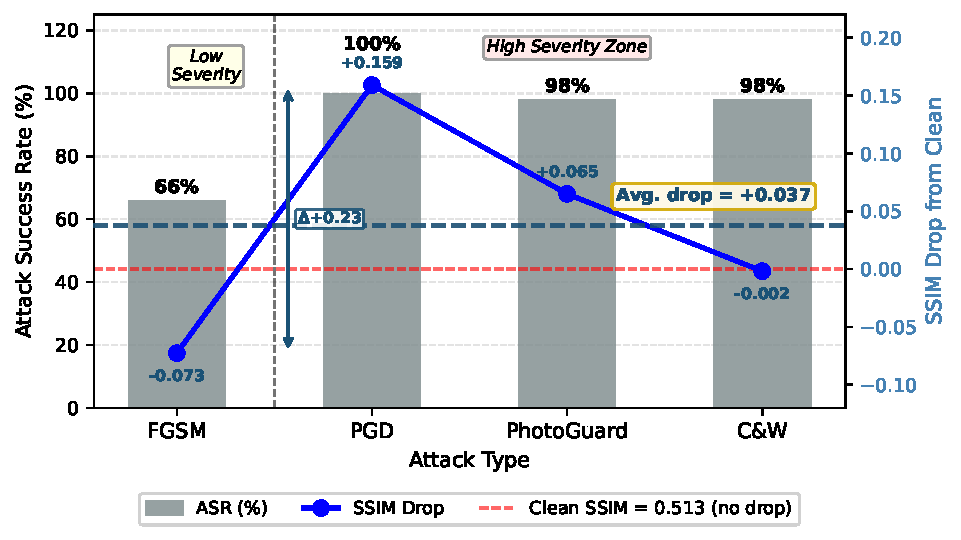
\includegraphics[width=0.84\linewidth]{figures/fig1_attack_severity.pdf}
  \caption{Attack severity on COCO-50: ASR$\downarrow$ bars (left; lower
  = defense working) and SSIM drop from clean baseline (right; larger drop
  = greater degradation). PGD achieves 100\% ASR; even FGSM reaches 66\%.}
  \label{fig:attack_severity}
\end{figure}

Adversarial defenses fall into three categories: (1)~detection and rejection
\cite{costa2024deep}; (2)~model hardening via adversarial training
\cite{madry2018towards}; and (3)~input preprocessing \cite{guo2018countering},
which requires no model modification. DiffPure \cite{nie2022diffusion} is the
leading preprocessing defense, applying a pixel-domain forward-reverse diffusion
pass; however, it achieves only 9.4\% average recovery on COCO-50.

In this work we propose \textbf{L-SHIELD}, a latent-space defense that
intercepts adversarial perturbations \emph{within} the VAE bottleneck.
Unlike global outlier rejection (a single threshold across all dimensions),
L-SHIELD pre-computes \emph{per-position} $(\mu,\sigma)$ for each of the
$4\!\times\!64\!\times\!64$ VAE latent positions, enabling correction targeted
precisely to adversarial anomalies while leaving clean positions unchanged. Our key contributions are: (1)~\textbf{L-SHIELD}, a no-retraining latent-space
defense that outperforms pixel-domain purification with negligible overhead;
(2)~\textbf{cross-attack generalization} across FGSM, PGD, PhotoGuard, and C\&W,
consistently beating DiffPure on FID and recovery rate; and
(3)~\textbf{cross-subset consistency}---identical 14.4\% average recovery on
both COCO-50 and COCO-50B without any dataset-specific tuning.

% =============================================================================
% SECTION II: PRELIMINARIES
% =============================================================================
\section{Preliminaries}

Latent Diffusion Models \cite{ho2020denoising,rombach2022high}, including
Stable Diffusion, compress an image into a latent code
$\mathbf{z}\!=\!\mathcal{E}(\mathbf{x})$ via a VAE encoder $\mathcal{E}$,
perform a forward Markov noising process on $\mathbf{z}$:
\begin{equation}
  q(\mathbf{x}_t \mid \mathbf{x}_{t-1}) =
  \mathcal{N}\!\left(\mathbf{x}_t;\,\sqrt{1-\beta_t}\,\mathbf{x}_{t-1},\,
  \beta_t \mathbf{I}\right),
\end{equation}
then reverse-denoise and decode via $\mathcal{D}$. In the img2img pipeline,
the input is partially noised to $t_{\text{start}} < T$, conditioning the
model on its visual content. An adversarial attack constructs
$\mathbf{x}_e = \mathbf{x} + \boldsymbol{\delta}$ with
$\|\boldsymbol{\delta}\|_p \leq \epsilon$ so that the pipeline output
$\mathcal{G}(\mathbf{x}_e)$ degrades relative to $\mathcal{G}(\mathbf{x})$.
We define the Attack Success Rate (ASR) as the fraction of images with SSIM
below $\tau\!=\!0.7$ \cite{salman2023raising}, and evaluate four white-box
attacks \cite{costa2024deep}: FGSM \cite{goodfellow2015explaining} (single-step,
$\epsilon\!=\!0.063$), PGD \cite{madry2018towards} (10-step iterative,
$\epsilon\!=\!0.063$), C\&W \cite{carlini2017evaluating} (optimization-based,
$\ell_2$ norm), and PhotoGuard \cite{salman2023raising} (encoder-targeted,
$\ell_\infty\!=\!0.126$).
This selection spans a deliberate attack taxonomy---single-step gradient, iterative
gradient, $\ell_2$-optimization, and VAE-encoder targeting---stress-testing
whether L-SHIELD generalizes across fundamentally different threat strategies
rather than overfitting to one; PhotoGuard is especially diagnostic since it attacks
the same latent bottleneck L-SHIELD defends (Sections~III-B and~IV-B).

% =============================================================================
% SECTION III: PROPOSED DEFENSE
% =============================================================================
\section{Proposed Defense: L-SHIELD}
\enlargethispage{30pt}

\subsection{Overview}

\begin{figure*}[t]
  \centering
  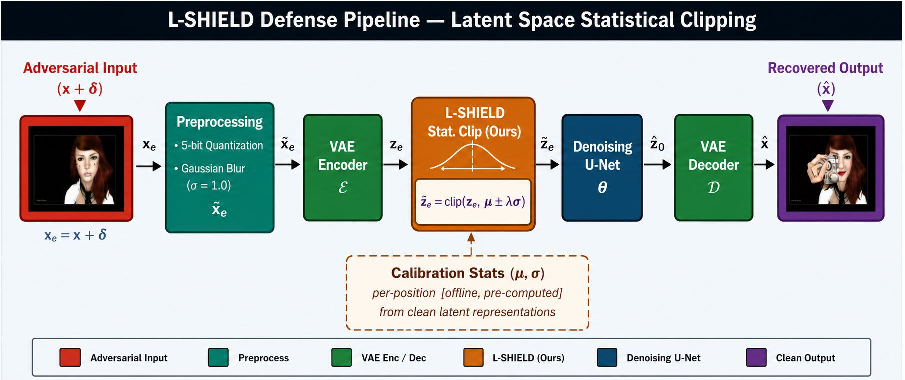
\includegraphics[width=0.96\textwidth]{figures/fig6_system_architecture.pdf}
  \caption{L-SHIELD pipeline: adversarial input $\mathbf{x}{+}\boldsymbol{\delta}$
  is preprocessed (5-bit quantization + Gaussian blur $\sigma{=}1.0$),
  encoded to latent $\mathbf{z}_e$, clipped per-position using offline
  statistics $(\boldsymbol{\mu}\pm\lambda\boldsymbol{\sigma})$ to yield
  $\hat{\mathbf{z}}_e$, then denoised by U-Net $\boldsymbol{\theta}$ and
  decoded to recovered output $\hat{\mathbf{x}}$.}
  \label{fig:arch}
\end{figure*}

L-SHIELD intercepts adversarial corruption at the VAE bottleneck through two
phases: an offline \emph{calibration} that pre-computes per-position
$(\boldsymbol{\mu},\boldsymbol{\sigma})$ from clean images once, and an
\emph{inference} step that clips any latent activation beyond the 3-sigma
boundary---preserving ${\approx}99.7\%$ of clean activations with no retraining.

Fig.\,\ref{fig:arch} traces the L-SHIELD inference pipeline left to right.
The \emph{adversarial input} block (crimson) shows $\mathbf{x}{+}\boldsymbol{\delta}$
with a real COCO-50 PGD-attacked thumbnail from our evaluation set, grounding
the diagram in actual experimental conditions. Before latent encoding, two
preprocessing steps attenuate adversarial structure: 5-bit quantization
discretizes pixel values to 32 levels, removing the fine floating-point
resolution adversarial perturbations exploit; and Gaussian blur ($\sigma{=}1.0$)
smooths residual high-frequency energy before the VAE encoder can amplify it
into latent-space outliers. The \emph{VAE Encoder} (forest-green) maps the
preprocessed image to $\mathbf{z}_e\!\in\!\mathbb{R}^{h\times w\times c}$
at 8$\times$ spatial downsampling.

The \emph{L-SHIELD block} (burnt-orange) is the only deviation from the
standard img2img pipeline. Its interior shows a Gaussian bell curve whose
central tan-shaded region---bounded by dashed lines at $\pm\lambda\sigma$---marks
positions with $|s_{h,w,c}|\leq\lambda$ passed through unchanged; the unshaded
tails beyond those boundaries are clipped to
$\boldsymbol{\mu}\pm\lambda\boldsymbol{\sigma}$, formalized by the
$\hat{\mathbf{z}}_e=\mathrm{clip}(\mathbf{z}_e,\boldsymbol{\mu}\pm\lambda\boldsymbol{\sigma})$
formula box. The corrected latent passes through the unmodified U-Net
$\boldsymbol{\theta}$ and decoder $\mathcal{D}$ to produce recovered output
$\hat{\mathbf{x}}$, shown alongside the input for direct before/after comparison.
The \emph{Calibration Stats} box (dashed amber, positioned \emph{below} the
pipeline to signal its offline nature) stores per-position
$(\boldsymbol{\mu},\boldsymbol{\sigma})$ computed once from $N{=}50$ clean
images; at inference, a read-only lookup adds \textbf{zero runtime overhead}
beyond one elementwise clip---in contrast to DiffPure~\cite{nie2022diffusion},
which runs a full forward-reverse diffusion pass at \emph{every} inference step.

\subsection{Vulnerability of Diffusion Models in Latent Space}
\label{sec:vulnerability}

The VAE encoder is a critical vulnerability surface \cite{salman2023raising,
costa2024deep}: pixel-small perturbations can be dramatically amplified in the
latent representation. Quantifying this on COCO-50, PGD generates the
highest outlier rate (2.53\% of positions beyond 3-sigma, mean deviation 3.52,
max 7.54); C\&W produces 2.35\% outlier positions (max 6.45); FGSM generates
fewer (0.38\%); and PhotoGuard, targeting the encoder directly, achieves the
largest per-position deviation (max 3.63) at only 0.06\% outlier rate.
These signatures motivate latent-space intervention: adversarial effects are
detectable and suppressible without disrupting clean semantics.

\subsection{Existing Defense Strategies}

Prior defenses fall into three categories: (1)~input transformations
\cite{guo2018countering} (lightweight but model-agnostic); (2)~model
hardening \cite{madry2018towards,papernot2016distillation} (impractical for
large generative models, as retraining is prohibitively expensive
\cite{athalye2018obfuscated}); (3)~detection \cite{costa2024deep} (cannot
recover the intended output); and (4)~purification \cite{song2018pixeldefend,
nie2022diffusion}, which reconstructs a clean input before model inference.
DiffPure \cite{nie2022diffusion}, the leading purification defense, applies a
pixel-domain forward-reverse diffusion pass, yet achieves only 9.4\% average
recovery on COCO-50. Related latent-space methods address distinct problems:
QSilk~\cite{rychkovskiy2025qsilk} clips activations for image quality (not
adversarial defense); VillanDiffusion~\cite{chou2023villandiffusion} evaluates
fixed $[-1,1]$ clipping for backdoor countermeasures; LQ-VAE~\cite{kyatham2019variational}
projects inputs onto a quantized manifold; and Def-VAE~\cite{li2025defvae}
uses per-class boundaries to \emph{detect} adversarial inputs---none recovers
the output image. L-SHIELD uniquely combines $(\mu,\sigma)$-calibrated
per-position clipping with full output recovery.

\subsection{L-SHIELD Algorithm}

\label{sec:algorithm}
During calibration, per-position $(\mu_{h,w,c},\sigma_{h,w,c})$ are computed from
$N$ clean encodings. At inference, the preprocessed input is encoded to
$\mathbf{z}_e\!=\!\mathcal{E}(\mathbf{x}_e)$ and each position evaluated by
\begin{equation}
  s_{h,w,c} = \frac{z_e^{(h,w,c)} - \mu_{h,w,c}}{\sigma_{h,w,c}},
\end{equation}
and clipped to the 3-sigma clean-distribution boundary:
\begin{equation}
  \hat{z}^{(h,w,c)} =
  \begin{cases}
    \mu_{h,w,c} + \lambda\,\sigma_{h,w,c} & \text{if } s_{h,w,c} > \lambda \\
    \mu_{h,w,c} - \lambda\,\sigma_{h,w,c} & \text{if } s_{h,w,c} < -\lambda \\
    z_e^{(h,w,c)} & \text{otherwise.}
  \end{cases}
\end{equation}
The corrected latent is decoded as
$\hat{\mathbf{x}}\!=\!\mathcal{D}(\mathrm{Denoise}_\theta(\hat{\mathbf{z}}_e))$.

Algorithm~\ref{alg:lshield} provides the complete pseudocode.
With $\lambda\!=\!3$, the boundary retains 99.73\% of clean activations
unmodified---the standard three-sigma Gaussian bound, which is theoretically
optimal for discriminating in-distribution from adversarially-shifted latents.
Calibration statistics stabilize rapidly with $N$, since per-position
distributions reflect the VAE encoder's fixed architecture rather than image
content.

\begin{algorithm}[t]
\caption{L-SHIELD Defense}
\label{alg:lshield}
{\small
\begin{algorithmic}[1]
\REQUIRE Clean images $\{\mathbf{x}^{(i)}\}_{i=1}^{N}$, encoder $\mathcal{E}$,
  decoder $\mathcal{D}$, denoiser $\theta$, threshold $\lambda{=}3$
\STATE \textit{Calibration:} $\mu_{h,w,c}\!=\!\frac{1}{N}\sum_i z^{(i)}_{h,w,c}$,
  $\sigma_{h,w,c}$; $\mathbf{z}^{(i)}\!=\!\mathcal{E}(\mathbf{x}^{(i)})$
\STATE \textit{Preprocess:} 5-bit quantization + Gaussian blur ($\sigma{=}1.0$) on $\mathbf{x}_e$
\STATE \textit{Encode:} $\mathbf{z}_e \leftarrow \mathcal{E}(\mathbf{x}_e)$
\FORALL{positions $(h,w,c)$}
  \STATE $s \leftarrow (z_e^{(h,w,c)} - \mu_{h,w,c})\,/\,\sigma_{h,w,c}$
  \IF{$|s| > \lambda$}
    \STATE $\hat{z}^{(h,w,c)} \leftarrow \mu_{h,w,c} + \mathrm{sign}(s)\cdot\lambda\,\sigma_{h,w,c}$
  \ELSE
    \STATE $\hat{z}^{(h,w,c)} \leftarrow z_e^{(h,w,c)}$
  \ENDIF
\ENDFOR
\RETURN $\mathcal{D}\!\left(\mathrm{Denoise}_{\theta}(\hat{\mathbf{z}}_e)\right)$
\end{algorithmic}
}
\end{algorithm}

\subsection{Effectiveness of L-SHIELD}
\label{sec:effectiveness}

L-SHIELD achieves the largest improvements on attacks with the densest latent
outlier patterns: PGD (24.4\% recovery vs.\ DiffPure's 12.6\%), C\&W
(18.1\% vs.\ 8.5\%), and PhotoGuard (10.0\% vs.\ 5.5\%)---the encoder-targeting
attack whose latent corruption falls squarely within L-SHIELD's clipping domain. DiffPure leads on FGSM (10.8\% vs.\ 5.1\%) because
FGSM's single-step perturbations produce diffuse high-frequency noise that
pixel-domain smoothing suppresses effectively, while the low FGSM outlier
rate (0.38\%) gives statistical clipping little to correct.
Fig.\,\ref{fig:qualitative} shows one representative COCO-50 image; SSIM
annotations are averages over all 50 images.

\begin{figure*}[t]
  \centering
  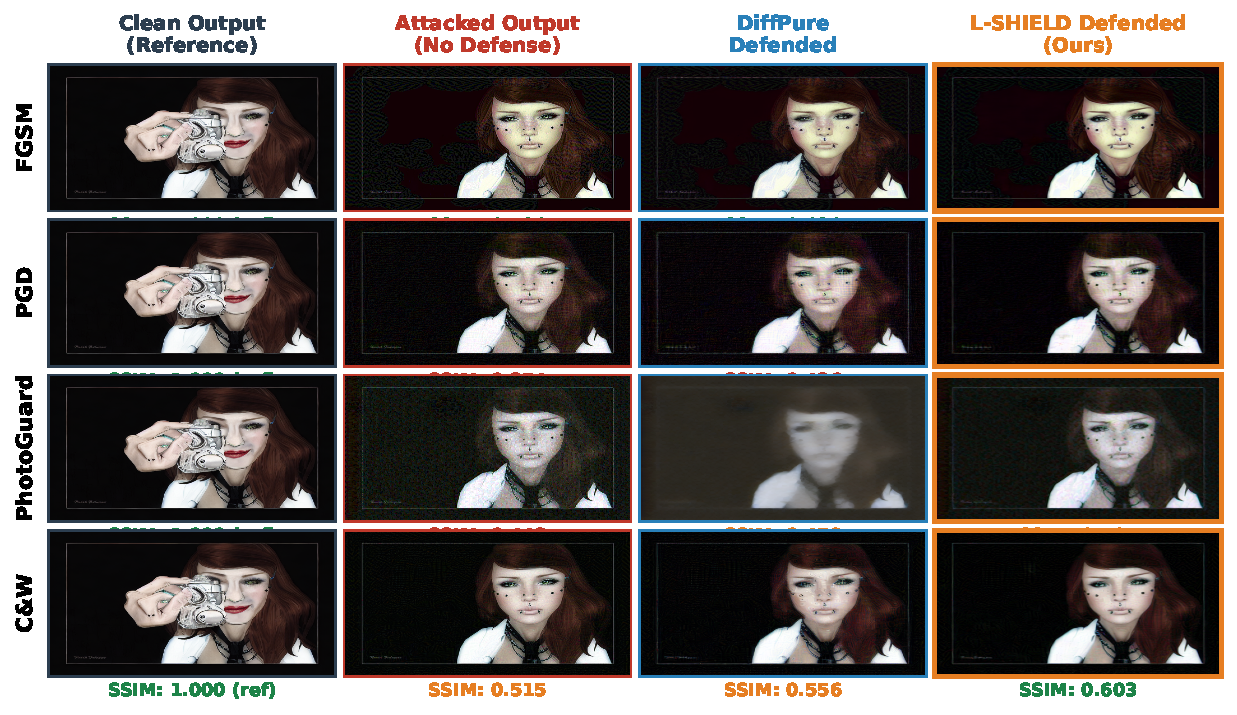
\includegraphics[width=0.96\textwidth]{figures/fig7_qualitative_samples.pdf}
  \caption{Qualitative comparison (COCO-50): Clean / Attacked / DiffPure /
  L-SHIELD (ours) across four attacks. SSIM annotated per cell (avg.\ 50
  images; higher SSIM = closer to Clean reference = better).
  L-SHIELD recovers most structure under PGD and C\&W.}
  \label{fig:qualitative}
\end{figure*}

% =============================================================================
% SECTION IV: EXPERIMENTAL EVALUATION
% =============================================================================
\section{Experimental Evaluation}

\subsection{Experimental Setup}

\textbf{Model and Pipeline.} All experiments use Stable Diffusion v1.5 in the
img2img configuration. The VAE encoder and decoder are kept frozen throughout;
no fine-tuning or retraining is performed for any defense.

\textbf{Datasets.} We use two disjoint 50-image subsets of the COCO val2017
validation set \cite{lin2014microsoft}: \textbf{COCO-50} (primary) and
\textbf{COCO-50B} (alternate IDs), enabling cross-subset evaluation without
dataset-specific tuning; all experiments were conducted on a high-end 48\,GB GPU.

\textbf{Metrics.} We report SSIM~\cite{wang2004image} ($\uparrow$),
PSNR ($\uparrow$), LPIPS~\cite{zhang2018unreasonable} ($\downarrow$),
ASR ($\downarrow$; fraction of images with SSIM\,$<$\,0.7 after defense),
FID~\cite{heusel2017gans} ($\downarrow$; distributional distance from clean),
and Recovery\% ($\uparrow$; fraction of attacked images restored above
SSIM\,0.7 by the defense). To evaluate multi-metric perceptual and structural
restoration simultaneously, we define a \textbf{Composite Quality Score}:
\begin{equation}
  \mathrm{Score}_{\mathrm{composite}} = \mathrm{SSIM} + \mathrm{PSNR}_{\mathrm{norm}} + (1 - \mathrm{LPIPS}),
\end{equation}
where $\mathrm{PSNR}_{\mathrm{norm}} = (\mathrm{PSNR} - \mathrm{PSNR}_{\min})/(\mathrm{PSNR}_{\max} - \mathrm{PSNR}_{\min})$
linearly rescales PSNR to $[0,1]$ across all evaluated scenarios ($[15.40, 21.29]\,\text{dB}$).
Since SSIM $\in [0,1]$ and $(1 - \mathrm{LPIPS}) \in [0,1]$, all three components contribute
equally to a maximum score of $3.0$. L-SHIELD is compared against
DiffPure~\cite{nie2022diffusion} (forward diffusion to $t\!=\!0.1T$,
full reverse denoising) and an undefended baseline.

\begin{figure*}[t]
  \centering
  \begin{minipage}[t]{0.48\textwidth}
    \centering
    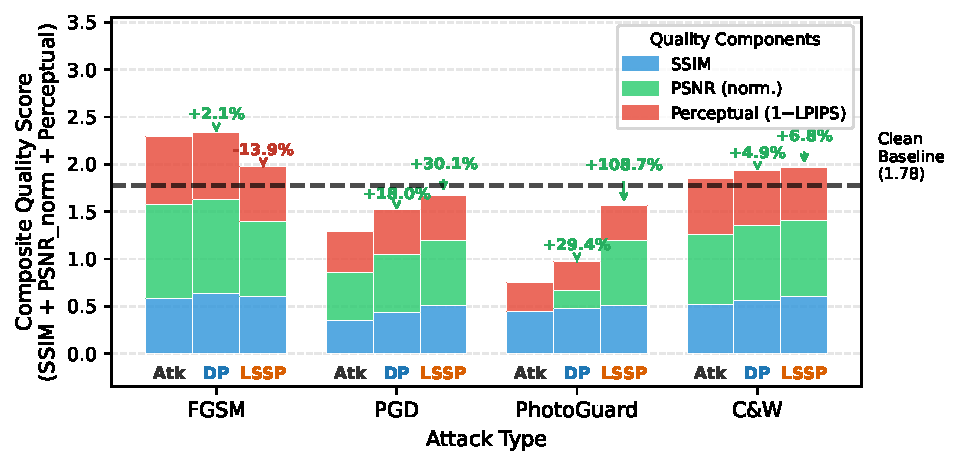
\includegraphics[width=\linewidth]{figures/fig4_stacked_quality.pdf}
    \caption{Composite Quality Score (SSIM + PSNR\textsubscript{norm} +
    (1\,--\,LPIPS)): Attacked (Atk), DiffPure (DP), L-SHIELD (LSSP).
    L-SHIELD exceeds clean baseline (1.78, dashed) on PGD, PhotoGuard, C\&W.}
    \label{fig:composite_quality}
  \end{minipage}
  \hfill
  \begin{minipage}[t]{0.48\textwidth}
    \centering
    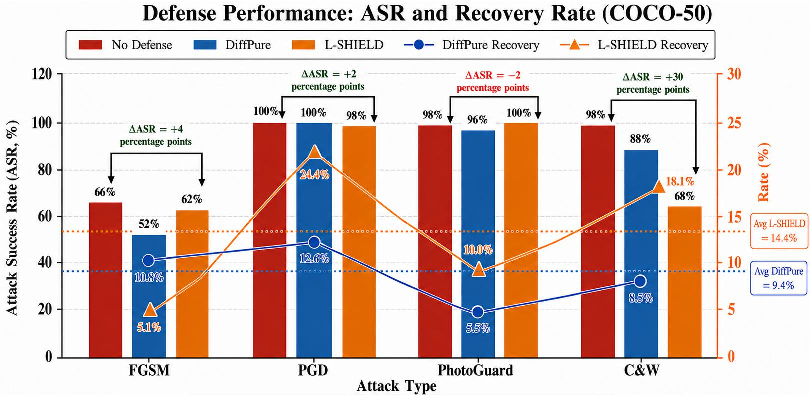
\includegraphics[width=\linewidth]{figures/fig2_defense_asr_recovery.pdf}
    \caption{ASR (bars) and Recovery\% (lines) on COCO-50. L-SHIELD leads on
    PGD (+24.4\%) and C\&W (+18.1\%); DiffPure marginally leads on FGSM.}
    \label{fig:defense_asr_recovery}
  \end{minipage}
\end{figure*}


\begin{table*}[t]
\caption{Defense Performance: SSIM$\uparrow$, ASR\%$\downarrow$,
Rec.\%$\uparrow$ Under Four White-Box Attacks on COCO-50 and COCO-50B.
Best result per row in \textbf{bold} (excluding No-Defense).
Recovery\% not applicable (--) for No-Defense rows.}
\label{tab:main_results}
\centering
\renewcommand{\arraystretch}{1.00}
\resizebox{\textwidth}{!}{%
\begin{tabular}{ll ccc ccc ccc}
\toprule
& &
\multicolumn{3}{c}{\textbf{No Defense}} &
\multicolumn{3}{c}{\textbf{DiffPure}~\cite{nie2022diffusion}} &
\multicolumn{3}{c}{\textbf{L-SHIELD (Ours)}} \\
\cmidrule(lr){3-5}\cmidrule(lr){6-8}\cmidrule(lr){9-11}
\textbf{Dataset} & \textbf{Attack} &
SSIM$\uparrow$ & ASR\%$\downarrow$ & Rec.\%\rlap{$^{\dag}$} &
SSIM$\uparrow$ & ASR\%$\downarrow$ & Rec.\%$\uparrow$ &
SSIM$\uparrow$ & ASR\%$\downarrow$ & Rec.\%$\uparrow$ \\
\midrule
\multirow{5}{*}{COCO-50}
  & FGSM       & 0.5859 & 66.0  & --  & \textbf{0.6305} & \textbf{52.0} & \textbf{10.8} & 0.6071 & 62.0  & 5.1 \\
  & PGD        & 0.3542 & 100.0 & --  & 0.4356 & 100.0 & 12.6 & \textbf{0.5117} & \textbf{98.0}  & \textbf{24.4} \\
  & PhotoGuard & 0.4483 & 98.0  & --  & 0.4786 & 96.0  & 5.5  & \textbf{0.5036} & 100.0 & \textbf{10.0} \\
  & C\&W       & 0.5151 & 98.0  & --  & 0.5564 & 88.0  & 8.5  & \textbf{0.6030} & \textbf{68.0}  & \textbf{18.1} \\
  & \textit{Average} & \textit{0.4759} & \textit{90.5} & \textit{--} &
    \textit{0.5253} & \textit{84.0} & \textit{9.4} &
    \textbf{\textit{0.5564}} & \textbf{\textit{82.0}} & \textbf{\textit{14.4}} \\
\midrule
\multirow{5}{*}{COCO-50B}
  & FGSM       & 0.6556 & 52.0  & --  & \textbf{0.6799} & \textbf{50.0} & \textbf{7.1} & 0.6451 & 62.0  & $-$3.0 \\
  & PGD        & 0.3824 & 100.0 & --  & 0.4532 & 100.0 & 11.5 & \textbf{0.5261} & \textbf{100.0} & \textbf{23.3} \\
  & PhotoGuard & 0.4186 & 100.0 & --  & 0.4550 & 98.0  & 6.3  & \textbf{0.5260} & 100.0 & \textbf{18.5} \\
  & C\&W       & 0.5481 & 98.0  & --  & 0.5824 & 88.0  & 7.6  & \textbf{0.6332} & \textbf{66.0}  & \textbf{18.8} \\
  & \textit{Average} & \textit{0.5012} & \textit{87.5} & \textit{--} &
    \textit{0.5426} & \textit{84.0} & \textit{8.1} &
    \textbf{\textit{0.5826}} & \textbf{\textit{82.0}} & \textbf{\textit{14.4}} \\
\bottomrule
\end{tabular}}
\end{table*}

\subsection{Defense Performance Against Adversarial Attacks}

Table~\ref{tab:main_results} presents the complete defense performance
comparison. Across both datasets, all four attacks consistently degrade the
Stable Diffusion img2img output, with PGD achieving the most severe structural
damage (SSIM 0.354 on COCO-50 and 0.382 on COCO-50B).


Fig.\,\ref{fig:defense_asr_recovery} uses a dual-axis design: grouped bars
(left $y$-axis) show ASR\%---lower is better---while lines with markers
(right $y$-axis) show Recovery\%---higher is better. Each attack cluster
contains three bars: grey (no defense), blue (DiffPure), and orange (L-SHIELD).
Dotted horizontal lines at the right margin mark per-method average Recovery\%
across all four attacks---9.4\% for DiffPure and 14.4\% for L-SHIELD---serving
as macro-level anchors. The \textbf{+pp} annotations above L-SHIELD bars
quantify ASR reduction relative to no-defense
($\Delta_{\mathrm{ASR}} = \mathrm{ASR}_{\text{no-def}} - \mathrm{ASR}_{\text{L-SHIELD}}$):
$+30$\,pp for C\&W ($98\%{\to}68\%$), $+4$\,pp for FGSM, and $+2$\,pp for
PGD---the latter genuine latent correction at the 100\% ceiling, confirmed by
the simultaneous 24.4\% Recovery\% gain and SSIM rise from 0.354 to 0.512.

The PhotoGuard case ($+0$\,pp) illustrates why both axes are necessary.
ASR is a binary threshold crossing: an image that goes from SSIM\,0.45 to
SSIM\,0.69 still registers as an attack success even though quality improved
substantially. Recovery\% is a graded measure that captures this partial
restoration. PhotoGuard targets the VAE encoder directly, preventing ASR
reduction regardless of latent clipping; yet L-SHIELD still improves structural
quality for nearly twice as many images as DiffPure (10.0\% vs.\ 5.5\%),
visible only on the Recovery\% axis.

L-SHIELD outperforms DiffPure on three of four COCO-50 attacks: PGD
(24.4\% vs.\ 12.6\%, $+94\%$ relative), C\&W (18.1\% vs.\ 8.5\%, $+113\%$;
highest post-defense SSIM 0.6030), and PhotoGuard (10.0\% vs.\ 5.5\%).
The FGSM exception (DiffPure leads: 10.8\% vs.\ 5.1\%) is explained in
Section~\ref{sec:effectiveness}. On COCO-50B, L-SHIELD similarly leads on PGD
(23.3\% vs.\ 11.5\%), PhotoGuard (18.5\% vs.\ 6.3\%), and C\&W (18.8\%
vs.\ 7.6\%); the FGSM $-3.0\%$ case motivates future adaptive threshold
selection. Gains are largest for the attacks with the densest latent outlier
patterns (PGD: 2.53\%, C\&W: 2.35\%), consistent with Section~\ref{sec:vulnerability}.

\subsection{FID Analysis}
\enlargethispage{25pt}

\begin{figure}[t]
  \centering
  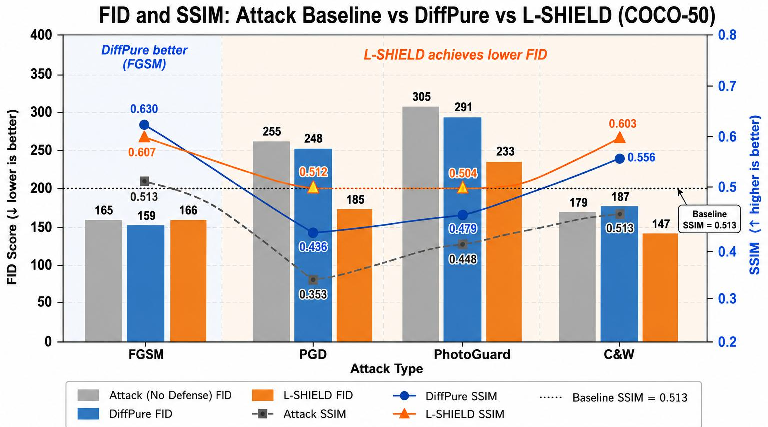
\includegraphics[width=0.78\linewidth]{figures/fig3_fid_ssim_tradeoff.pdf}
  \caption{FID$\downarrow$ (bars; lower = better) and SSIM$\uparrow$ (lines;
  higher = better) on COCO-50. Shaded columns: L-SHIELD FID $<$ DiffPure.
  L-SHIELD reduces average FID 221.1$\to$182.7 ($-$17.4\%).}
  \label{fig:fid_ssim}
\end{figure}

Table~\ref{tab:fid_results} and Fig.\,\ref{fig:fid_ssim} present the FID
analysis. The dual-axis figure pairs FID bars (left axis, lower is better:
distributional distance from clean outputs) with SSIM lines (right axis,
higher is better: per-image structural fidelity), together revealing whether
a defense improves global realism at the cost of per-pixel fidelity---a
trade-off neither metric alone can detect. Three of four attack columns are
shaded orange, marking where L-SHIELD achieves lower FID than DiffPure.
The black dotted line at SSIM\,=\,0.513 marks the undefended clean-image
output baseline; any defended value above it reflects genuine quality
improvement beyond the unattacked pipeline. Both DiffPure and L-SHIELD
exceed this ceiling on FGSM and C\&W, while the un-shaded FGSM column
reflects the low latent outlier rate (0.38\%) discussed in
Section~\ref{sec:vulnerability}: L-SHIELD's correction has little to act on
there, whereas DiffPure's Gaussian front-end suits FGSM's mild additive
noise regime.

% --- Table II ---
\begin{table}[t]
\caption{Fr\'{e}chet Inception Distance (FID~$\downarrow$) Across Attacks
and Defenses. Best FID per column in \textbf{bold}.}
\label{tab:fid_results}
\centering
\renewcommand{\arraystretch}{1.04}
\resizebox{\linewidth}{!}{%
\begin{tabular}{llccccc}
\toprule
\textbf{Dataset} & \textbf{Defense} &
\textbf{FGSM} & \textbf{PGD} & \textbf{PGuard} & \textbf{C\&W} & \textbf{Avg} \\
\midrule
\multirow{3}{*}{COCO-50}
  & Attack (No Def.) & 165.3 & 255.0 & 305.3 & 179.0 & 226.1 \\
  & DiffPure~\cite{nie2022diffusion} & \textbf{158.5} & 248.3 & 290.5 & 187.2 & 221.1 \\
  & L-SHIELD (Ours)  & 166.3 & \textbf{185.2} & \textbf{232.6} & \textbf{146.7} & \textbf{182.7} \\
\midrule
\multirow{3}{*}{COCO-50B}
  & Attack (No Def.) & 117.2 & 248.9 & 317.1 & 162.9 & 211.5 \\
  & DiffPure~\cite{nie2022diffusion} & \textbf{121.5} & 246.7 & 285.7 & 161.5 & 203.9 \\
  & L-SHIELD (Ours)  & 129.8 & \textbf{193.8} & \textbf{213.0} & \textbf{127.9} & \textbf{166.1} \\
\bottomrule
\end{tabular}}
\end{table}

L-SHIELD achieves average FID 182.7 vs.\ 221.1 for DiffPure (\textbf{17.4\%}),
with gains on COCO-50B confirming cross-subset consistency (166.1 vs.\ 203.9,
18.5\%). For PhotoGuard---which targets the VAE encoder directly---L-SHIELD
reduces FID from 305.3 to 232.6 (23.8\%); DiffPure achieves only 4.8\%
(to 290.5), as pixel-domain denoising cannot undo encoder-level corruption.

\subsection{Cross-Subset Generalization}
\enlargethispage{20pt}

\begin{figure}[b]
  \centering
  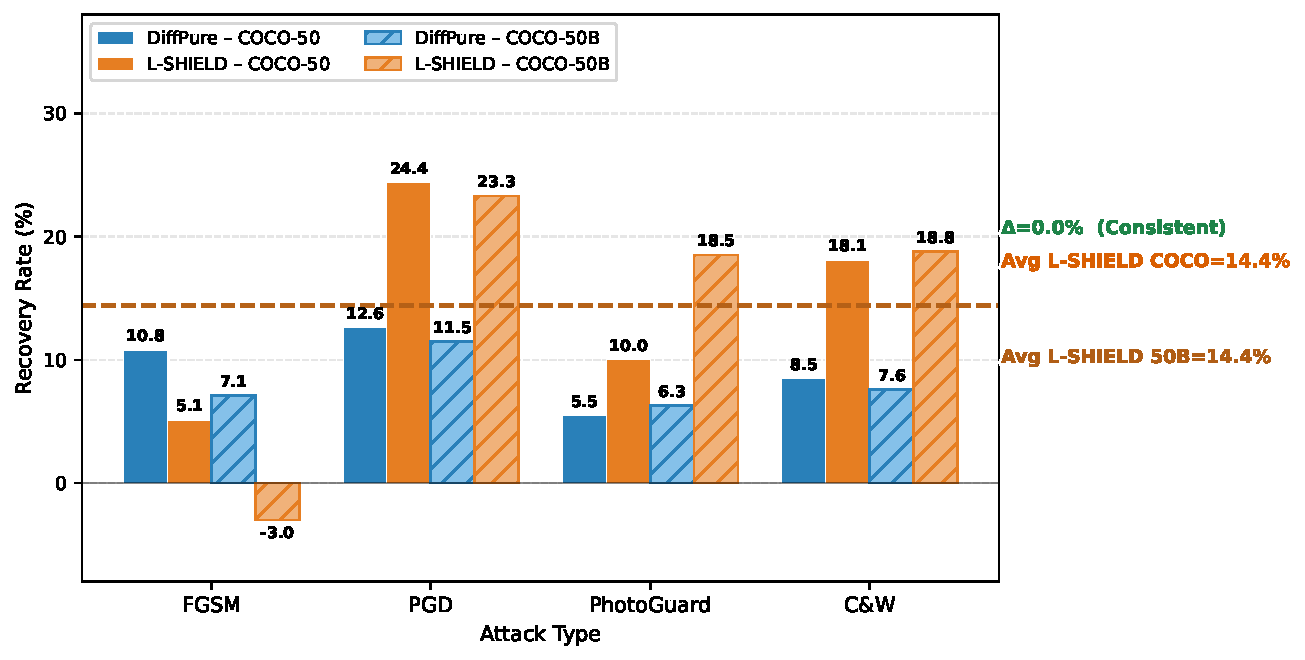
\includegraphics[width=0.78\linewidth]{figures/fig5_cross_dataset.pdf}
  \caption{Cross-subset Recovery\%$\uparrow$: COCO-50 (solid) vs.\ COCO-50B
  (hatched). L-SHIELD achieves identical 14.4\% average on both;
  DiffPure declines 9.4\%$\to$8.1\%.}
  \label{fig:cross_dataset}
\end{figure}

As shown in Fig.\,\ref{fig:cross_dataset}, L-SHIELD achieves identical 14.4\%
average recovery on both subsets without subset-specific tuning, versus
DiffPure's 9.4\% (COCO-50) and 8.1\% (COCO-50B), with FID improvements of
17.4\% and 18.5\% respectively. Both subsets are drawn from COCO val2017, so
this measures within-distribution robustness across disjoint image sets.
The consistency reflects that per-position $(\mu,\sigma)$ calibration captures
the VAE encoder's architecture-intrinsic latent structure rather than
content-specific features of any individual image set.

% =============================================================================
% SECTION V: COMPARISON WITH EARLIER WORKS
% =============================================================================
\section{Comparison with Earlier Works}
\enlargethispage{30pt}

Table~\ref{tab:comparison} summarizes the comparison.
L-SHIELD outperforms DiffPure by 53\% in recovery, 17.4\% in FID, and 5.9\%
in SSIM---all without retraining---confirming that latent-domain correction
is most effective against attacks producing dense latent-space corruption (PhotoGuard, PGD).

\enlargethispage{12pt}
% --- Table III ---
\begin{table}[t]
\caption{Comparison with Prior Defenses on COCO-50 (averages across all four
attacks). Input Transform and Adversarial Training not evaluated on SD img2img.}
\label{tab:comparison}
\centering
\renewcommand{\arraystretch}{1.08}
\resizebox{\linewidth}{!}{%
\begin{tabular}{lccccc}
\toprule
\textbf{Method} & \textbf{Type} & \textbf{Retraining} &
\textbf{Avg Rec.\%} & \textbf{Avg FID} & \textbf{Avg SSIM} \\
\midrule
No Defense                    & --             & No  & --    & 226.1 & 0.476 \\
Input Transform~\cite{guo2018countering} & Preprocessing & No &
  \multicolumn{3}{c}{\textit{not evaluated in this study}} \\
Adversarial Training~\cite{madry2018towards} & Hardening & Yes &
  \multicolumn{3}{c}{\textit{not evaluated in this study}} \\
DiffPure~\cite{nie2022diffusion} & Diffusion Purif. & No & 9.4 & 221.1 & 0.525 \\
\textbf{L-SHIELD (Ours)}      & Latent Stat. Proj. & No & \textbf{14.4} & \textbf{182.7} & \textbf{0.556} \\
\bottomrule
\end{tabular}}
\end{table}

% =============================================================================
% LIMITATIONS AND CONCLUSION
% =============================================================================

\textbf{Limitations.}
Both subsets are from COCO val2017, demonstrating within-distribution robustness
but not cross-dataset generalization; FID at $n{=}50$ is indicative.
L-SHIELD degrades on FGSM in COCO-50B ($-3.0\%$) due to the sparse latent
outlier pattern (0.38\%, Section~\ref{sec:vulnerability}). The white-box threat model leaves
black-box robustness and architectures beyond SD~v1.5 as future work.

\section{Conclusion}
\enlargethispage{15pt}

L-SHIELD is a training-free per-position latent clipping defense achieving
a 53\% recovery improvement over DiffPure on COCO-50 (14.4\% vs.\ 9.4\%)
and a 17.4\% FID reduction (182.7 vs.\ 221.1), reproduced consistently on
COCO-50B. Its no-retraining design is compatible with any latent diffusion
pipeline and is especially effective against attacks producing dense latent-space corruption.

% =============================================================================
% ACKNOWLEDGMENT
% =============================================================================
\section*{Acknowledgment}
Removed for double-blind review.

% =============================================================================
% REFERENCES
% =============================================================================
\enlargethispage{30pt}
\IEEEtriggeratref{13}
\bibliographystyle{IEEEtran}
\footnotesize
\setlength{\bibsep}{0pt}
\vspace{-4pt}
\bibliography{references}

\end{document}
